%%%%%%%%%%%%%%%%%%%%%
%                                             %
%                 Experiment M-3              %
%               g with a pendulum             %
%                                             %
%%%%%%%%%%%%%%%%%%%%%

% Hyperref doesn't like math in chapter titles.
\iffalse
\labChapter{M}{The Measurement of $g$ with a Simple Pendulum}
\else
%\labChapter{M}{The Measurement of \textit{g} with a Simple Pendulum}
\labChapter{M}{Determination of Acceleration due to Gravity, \textit{g}, with Simple Pendulum}
\fi
\label{lab:M10}

% Introduction
%\section{Introduction}

%The acceleration due to gravity is determined by measuring the parameters of the nearly simple harmonic motion of a simple pendulum.  The construction of the pendulum and restrictions on the motion of the pendulum permit some simplifying assumptions to be used to derive a relationship for $g$ in terms of easily measured parameters.










% Background
\section{Background}

In this lab, the acceleration due to gravity is determined by measuring the parameters of the nearly simple harmonic motion of a simple pendulum.  The construction of the pendulum and restrictions on the motion of the pendulum permit some simplifying assumptions to be used to derive a relationship for $g$ in terms of easily measured parameters.

The gravitational attraction of the Earth on any massive body provides a force, which can accelerate a mass free to move under the influence of this force.  This acceleration $g$ is dependent on the mass of the earth and inversely on the distance of the mass from the center of the earth.  The value of $g$ is usually assumed to be constant over small vertical distances, i.e.\ distances that are small with respect to the distance to the center of the earth.  Thus we will compare our results to the measured value of $g$ at sea level.  The value at sea level in Fairfield is $g = 9.803\,\meter\per\second\squared$.

A pendulum is a massive body suspended such that it can swing freely.  In the general case, the mass of the pendulum is an extended mass and is called a physical pendulum.  An example of a physical pendulum might be a long piece of lumber, which is suspended from a nail through a hole near one end of the wood. This pendulum, when displaced sideways from its rest position, will swing back and forth under the influence of gravitational force which acts to restore the pendulum to its stationary hanging position.  The harmonic motion of the swinging pendulum must be analyzed carefully by considering torque on the pendulum and the pendulum's inertia.  The torque is the turning force produced by gravity and its inertia is the total effect of all the mass parts of the pendulum resisting rotation around the pivot.  The torque and inertia are exactly analogous to force and mass in the linear motion case described by Newton's Second Law, $F = m a$.

When all of the mass of the pendulum can be considered at a common distance from the pivot, then the physical pendulum is a simple pendulum.  An example of a simple pendulum is a relatively small, massive object suspended from a long, nearly massless connection to a pivot like a short, heavy bolt, tied to a pivot with a thin thread.

Under the assumption of a simple pendulum, the analysis of the motion can be carried out using Newton's Laws of Linear Motion that we have seen in class.  Fig.~\ref{M03Fig01} illustrates a simple pendulum at some arbitrary point in its swinging motion back and forth.  We define this point by the angle of the thread with the vertical, indicated by the dashed line.  The forces acting on the mass are its weight straight down and the tension in the thread.  The weight can be resolved into a component along the direction of the thread and a component perpendicular to the thread, i.e.\ along the tangent of the arc of the swing.

\begin{figure}
  \begin{center}  
    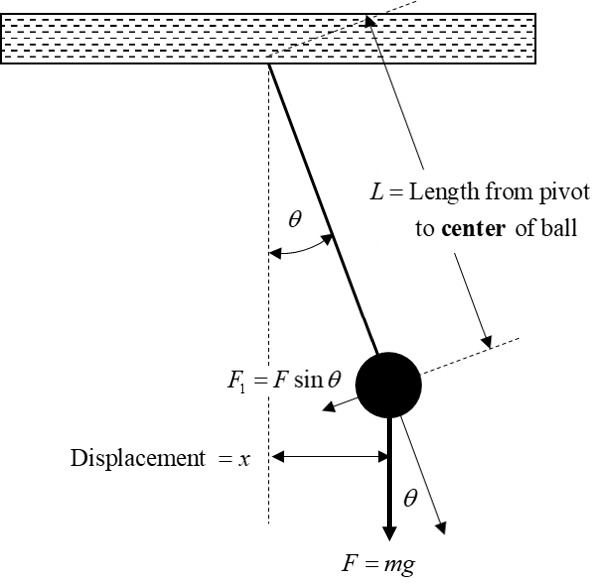
\includegraphics[width=4.0in]{Fall/Experiment03Figures/M10_figure1_squish_v01.png}
  \end{center}
  \caption{Force Diagram and variables used in Experiment M-\ref{lab:M3}.}
  \label{M03Fig01} % Goes AFTER caption
\end{figure}

$F_{1}$, the force along the direction of motion, is equal to $F \sin(\theta) = m g \sin(\theta)$.  We will now make a further simplifying assumption which is to assume that the maximum angular displacement, i.e.\ the maximum value of $x$ is small.  If the value of $x$ and therefore $\theta$ is small, then the magnitude of both the $\sin(\theta)$ and $\tan(\theta)$ are essentially equal to $\theta$, measured in radians.  For small angles then, the value of the $\sin(\theta) = x/L$.  The implication of this assumption is that the pendulum never swings very far from the vertical.  Therefore the restoring force, i.e.\ the force that is acting to return the pendulum to its equilibrium vertical position, is assumed to be acting horizontally.  This is clearly never true except at the equilibrium position where the restoring force is zero.  The implication of this assumption is that the actual restoring force is always less than the value we assume it to be.

The period of the pendulum is the time it takes to swing through a complete cycle, or one complete swing back to the starting point.  Using the small angle assumption described above, we can write the restoring force as
\[
	F = -m g \sin(\theta) = -m g \frac{x}{L}.
\]
The minus sign means that the restoring force is in the opposite direction from the displacement $x$.  When the restoring force of a system is of the form $F = -k x$, the system will oscillate in simple harmonic motion.

To see what this motion looks like we will use Newton's Second Law,
\begin{equation}
  \label{eq:M03fma}
  F = -m g \frac{x}{L} = m a
\end{equation}
where $a$ is the acceleration of the mass in the $x$-direction.
Substituting the definition of acceleration
\[
a = \frac{{\rm d}^2 x}{{\rm d} t^{2}}
\]
into Eqn.~\ref{eq:M03fma} yields an equation for displacement, $x$, as a function of time, $t$, namely
\[
-\frac{mg}{L} x(t) = m \frac{{\rm d}^2 x}{{\rm d} t^{2}}.
\]
Upon simplifying, the mass, $m$, disappears, yielding
\[
x(t) = -\left(\frac{L}{g}\right) \frac{{\rm d}^2 x}{{\rm d} t^{2}}.
\]
This second order, linear, differential equation has a solution
\[
x(t) = A \cos\left(2\pi \frac{t}{T} \right)
\]
where $A$, the amplitude, is the maximum value of $x$; $T$ is the period; and the motion is such that at $t = 0$, the pendulum is at its maximum displacement, i.e.\ $x = A$.  Note that the motion is independent of the mass.  Substitution of this solution into the differential equation yields an expression for the period as
\begin{equation}
  \label{eq:M03CalcTime}
  T = 2\pi \sqrt{\frac{L}{g}}.
\end{equation}
Rearranging this expression we obtain
\begin{equation}
  \label{eq:M03Calcg}
  g = 4\pi^2 \frac{L}{T^2}.
\end{equation}

Had we not constrained the motion of the pendulum to small amplitudes, the expression for the period would be given by
\begin{equation}
\label{eq:M03PeriodSeries_pendulum}
T = 2\pi \sqrt{\frac{L}{g}}  \left[ 1 +
  \frac{1}{ 4} \sin^2\left(\frac{\theta}{2}\right) +
  \frac{9}{64} \sin^4\left(\frac{\theta}{2}\right) + \ldots \right]
\end{equation}
Thus as the angle gets larger, the period increases.

When the pendulum swings with very small angles, the period is essentially independent of the amplitude.  However, from the more precise expression above for the period, this is not strictly true.  An amplitude decrease could result from the effects of friction in the pivot or air drag of the thread and mass.  Pendulum clock makers go to great pains to not only keep the length constant, but the amplitude of the swing as well.  Since we will average over many cycles, we must also assume that the amplitude does not change as we measure the period.  In our experiment, we might be tempted to average a very large number of cycles to reduce measurement errors.  However the necessarily larger initial amplitude together with the decreasing amplitude caused by friction effects would change the average period.  For the last case, we will do just that by deliberately start with a large amplitude and observe whether there is an increase in the measured period.

%\subsection{Case 2 Pendulum moving in a circle}
%
%In Case 2 you will explore the period with the pendulum moving in a circle.
%
%The radius of motion in terms of the length and the angle $\theta$ is $R=L\sin \theta$. The ball moves in a horizontal plane.
%Therefore its vertical component of acceleration is zero and the vertical forces must cancel.
%The vertical component of tension equals the weight of the ball, $F_T \cos\theta = M g$.
%
%The ball is in uniform circular motion around a horizontal circle.
%The centripetal force is
%\begin{equation}
%  F_r = F_T \sin\theta = M g \tan\theta = \frac{M v^2}{L \sin\theta}.
%\end{equation}
%Substituting $v= 2\pi L \sin(\theta)/T$ and solving for $g$ gives:
%\begin{equation}
%  \label{eq:M03circle}
%  g = \frac{4\pi^2 L}{T^2}\cos\theta.
%\end{equation}
%
%Using all your results other than Case 6 calculate the average and standard deviation for your experimental values of $g$ as shown in Eqn.~\ref{eq:errorSigmaX}.
%
%How does the difference of your result for Case 6 from your average $g$ compare with the standard deviation?















\section{Experimental Procedure}


\begin{enumerate}
\item \textbf{OVERALL GOALS:}
\begin{itemize}
    \item We study simple harmonic motion of a simple pendulum to derive acceleration due to gravity.
    \item The pendulum is the combination of both the string and the ball. The pendulum length is the distance from the pivot point to the center of mass of the ball (the center where force of gravity is overall acting upon). The total pendulum length can be determined from adding together the thread length $y$ and the ball radius as determined by:
\begin{itemize}
    \item Measuring thread length $y$ from pivot point to the top surface of the ball.
    \item Measuring diameter of the ball with calipers, and determining radius.
\end{itemize}
\end{itemize}


\item \textbf{Five Cases:} For this experiment, you will use thread lengths of approximately 50, 100, 130, and 170~\centi\meter. You don't have to set the lengths to be exactly those lengths. The point here is to cover a wide range to investigate how the motion is dependent on pendulum length. Get close and just make sure to measure the thread length carefully; record the measured value, and determine the total pendulum length for the given case. 
\begin{enumerate}
\item\label{step:M03Case1} $y\simeq  50\,\centi\meter$ with a small angle (displacement from rest of $\sim$1--3\degree, $\sim$1--2 inches, $\sim$1--2 finger knuckles).
%\item\label{step:M03Case2} $y\simeq  50\,\centi\meter$ Leave the length the same as Case~\ref{step:M03Case1} and use a small angle with circular motion.
%  \subitem -Leave the pendulum length the same as Case 1.
%  \subitem -Hold the weight displaced about 2~\centi\meter from its resting place.
%  \subitem -Give it a small initial velocity perpendicular to the displacement to make it move in a circle. Practice a few times to get it to move close to a circle.
\item\label{step:M03Case3} $y\simeq 100\,\centi\meter$ with a small angle.
\item\label{step:M03Case4} $y\simeq 130\,\centi\meter$ with a small angle.
\item\label{step:M03Case5} $y\simeq 170\,\centi\meter$ with a small angle.
\item\label{step:M03Case6} $y\simeq 170\,\centi\meter$ with a large angle.
  \subitem -Do not change the thread length in going from case~\ref{step:M03Case5} to case~\ref{step:M03Case6}.
  \subitem -Use an angle of approximately 45\degree--60\degree (a useful and consistent starting point that provides a large angle is the edge of the table).
\end{enumerate}

\item \textbf{NOTE ON NUMBER OF TRIALS:} For each of the five cases, each person will perform 5 time trials. Everyone can record at roughly the same time, but don't worry if you aren't all timing the exact same swings (i.e. someone starts a half or whole cycle late); just make sure to time a total of 10 cycles for each trial. By everyone taking data for 5 time trials each, a two-person group will end up with 10 total data points, and a three-person group will have 15 total data points for each case, etc.

\item Create a data table for the first case (this table can be copied/pasted for the additional cases):
\begin{itemize}
\item Common data for the entire experiment includes the ball diameter and the accepted $g$.
\item Common data for each case includes:
\begin{itemize}
  \item The case number
  \item The case description
  \item Measured thread length $y$
  \item Calculated pendulum length $L$
  \item Estimated uncertainty in length $\delta L$
  \item Approximate angle of displacement $\theta_\text{displacement}$
\end{itemize}
\item Create enough \textbf{rows} to include all time trials for your group
\item For each case, include \textbf{columns} for
  \begin{itemize}
  \item Measured \textbf{total time} of the 10 swings $t_{10\text{cycles}}$
  \item Estimated uncertainty in total time $\delta t_{10\text{cycles}}$
  \item Period $T$ derived from your measured time
  \item Uncertainty $\delta T$ derived from $\delta t_{10\text{cycles}}$
  \item Derived values for $g$ from small amplitude approximation Eqn.~\ref{eq:M03Calcg}
  \item Derived uncertainty $\delta g$
  \item Derived values for corrected value, $g_\text{corrected}$. Corrected by incorporating the smaller terms of the series in Eqn.~\ref{eq:M03PeriodSeries_pendulum}. Obtained by multiplying by the square of the factor in square brackets.
  \item Include \textbf{additional rows} for:
  \begin{itemize}
    \item $T_\text{avg}$: Average $T$ fromo all trials of the current case
    \item $g_{\text{avg}}$: Average $g$ from all trials of the current case
    \item $\delta g_{\text{avg}}$: Average uncertainty of $g$ from all trials of the current case
    \item $g_\text{corrected,avg}$: Average corrected values of $g$
    \item Difference between $g_{\text{avg}}$ and the accepted $g$
  \end{itemize}

  
%    \subitem For each trials, record the total time, the average period and the calculated value of $g$ from Eqn.~\ref{eq:M03Calcg}.
  %\item Calculate the average and standard deviation of $g$ for the case from the ten trials.
%  \item Calculate the difference $\delta g$ between your average value for the case and the accepted $g$.
%  \item Compare $\delta g$ to the expected error based on the standard deviation for the case.
  \end{itemize}
  
%  \item Compute the average and standard deviation of your measured values of $g$ for each case.

    \end{itemize}




%\item \textbf{DATA TAKING:}
%\begin{itemize}
\item Measure the thread length $y$. Attach one end of the thread to the provided pendulum clamp in such a way that you can accurately measure the distance from the pivot to the top surface of the ball. Set the length of the thread approximately to the value for the case (doesn't have to be exact, we're just going for a range of lengths across the cases).
\item Add the radius of the ball to the thread length to establish the pendulum length $L$. Estimate and note the uncertainty in the pendulum length $\delta L$.
\item Note the approximate angle of displacement $\theta_\text{displacement}$ from rest position:
    \begin{itemize}
        \item For cases~\ref{step:M03Case1} -- ~\ref{step:M03Case5}, the starting displacement should be small (e.g. 4\% of $L$, as described above with the approximate thread lengths).
        \item For case~\ref{step:M03Case6}, use a large angle of approximately 45\degree -- 60\degree~(like the edge of the table described earlier).
    \end{itemize}
\item For each case, perform 5 time trials per person (i.e. 10 or 15 total data points per two- or three-person group as mentioned above) as follows:
  \begin{itemize}
  \item Measure the time $t_{10\text{cycles}}$ for 10 cycles of the pendulum. One cycle is going from the pendulum's initial position, swings out, swings back to its initial position.
    \begin{itemize}
        \item Start and stop the stopwatch at one end of a swing where the velocity is zero. It is better not to start the watch as you release the mass, but rather at a later point where $v = 0$. This will insure that your starting point is a $v = 0$ point rather than not because of an initial velocity given to the ball when you release it. 
        \item Count one cycle as the mass returns to the starting point, i.e. after one complete swing out and back.
        \item Suggestion for counting: Index your counting by starting at 0. Starting the stopwatch at 0 and stopping when you say 10 will give you 10 full cycles.
    \end{itemize}
  \item Estimate your time trial uncertainty $\delta t_{10\text{cycles}}$ based on your reaction time (generally ranging $\sim$0.150 -- 0.300 seconds) and your stopwatch precision. (i.e. results are $t_{10\text{cycles}} \pm \delta t_{10\text{cycles}}$). \textit{CONSIDER}: Where do the uncertainties come from?
  \item Determine the period $T$ for one cycle from each time trial of ten cycles.
  \item Similarly, determine the period uncertainty $\delta T$ for one cycle from each time trial. (Hint: how many cycles did you observe?)
  \item Calculate the value of $g$ for each time trial using the small amplitude approximation, Eqn.~\ref{eq:M03Calcg}.
  \item Similarly, determine the uncertainty of your value for $g$ by making $g$ as large as your uncertainty allows and subtract the original value; the difference is the uncertainty in $g$. In other words, maximize $g_{\text{maximize}}$ with a smaller period and larger pendulum length: using ($T - \delta T$) as the period and ($L + \delta L$) to make $g_{\text{maximize}}$ bigger by dividing by a smaller period and multiplying by a longer length). Then get the uncertainty by $\delta g = g_{\text{maximize}} - g$.
  \subitem \begin{equation}
  \label{eq:M03Calcg_subitem_maximized}
  g_{\text{maximize}} = 4\pi^2 \frac{(L + \delta L)}{(T - \delta T)^2}
\end{equation}
\item Calculate the corrected value, $g_\text{corrected}$, by including the next two terms of the series according to Eqn.~\ref{eq:M03PeriodSeries_pendulum} obtained by multiplying by the square of the factor in square brackets. This is like Eqn.~\ref{eq:M03Calcg} becoming:
  \subitem \begin{equation}
  \label{eq:M03Calcg_subitem_corrected}
  g = 4\pi^2 \frac{L}{T^2} \left[ 1 +
  \frac{1}{ 4} \sin^2\left(\frac{\theta}{2}\right) +
  \frac{9}{64} \sin^4\left(\frac{\theta}{2}\right) \right]^2
\end{equation}
  %\end{itemize}
  \begin{itemize}
  \item Calculate your average values from everyone's trials for the current case:
      \item $T_\text{avg}$, the average value of $T$
      \item $g_{\text{avg}}$, the average value of $g$
      \item $\delta g_{\text{avg}}$, the average uncertainty of $g$
      \item $g_\text{corrected,avg}$, the average corrected value of $g$
  \end{itemize}
  \end{itemize}
  \item Calculate the difference between $g_{\text{avg}}$ and the accepted $g$
%\item Calculate the average and standard deviation of $g$ from the 10 trials.
%\item Calculate the expected error in your average value of $g$ for the case.
%\item Compare this expected error to the difference between the accepted value of $g$ and the average value for the case.
\item Compare your value for $g \pm \delta g$ to the difference between the accepted value of $g$ and the average value for the case. \textit{DISCUSSION POINT}: Do your experimental values for $g$ agree with the accepted value of $g$. In other words, does $g \pm \delta g$ overlap with the accepted value by covering the difference between the experimental and actual values?
%\end{itemize}



%  \item Now analyze the overall results of the experiment. \textbf{For each case} create a row in your data layout that includes:
%  \begin{itemize}
%    \item the average period for the case.
%    \item the average measured value of $g$ using the small amplitude approximation, Eqn.~\ref{eq:M03Calcg}.
%    \item the corrected average measured value of $g$ corrected according to Eqn.~\ref{eq:M03PeriodSeries_pendulum} obtained by multiplying by the square of the factor in square brackets.
  %  \item the standard deviation of the measured value of $g$,
  %  \item the difference between the measured value and the accepted value of $g$,
  %\end{itemize}
%\end{itemize}


\item{\textbf{Graphical Analysis:}}

\begin{itemize}
\item Using data from the four small amplitude cases (Cases~\ref{step:M03Case1}--~\ref{step:M03Case5}), plot the square of the average period, $T^2$, as a function of the length $L$. \textbf{Do not} use the large angle Case~\ref{step:M03Case6}.
\item Plot all data points from your lab group and draw the best fit straight line through your data points (force the fit to pass through the origin).
\item Determine the slope of your graph.
\item From the expression for the period, the measured slope, $m$, should give you your best estimate of the value of $g$.  Since the expression for $T^2$ is given by
  \begin{equation}
    \label{eq:M03slope}
    T^2 = \frac{4\pi^2}{g} L
  \end{equation}
  the slope of your graph, $m = 4\pi^2/g$.  Thus your final value for $g_\text{slope}$ is $4\pi^2/m$.
  
!!!!!!!!!!!!!! Add in actual uncertainty from the slope?

  !!!!!!!!!!!!!! Add in actual uncertainty from the slope?


!!!!!!!!!!!!!! Add in actual uncertainty from the slope?


!!!!!!!!!!!!!! Add in actual uncertainty from the slope?


!!!!!!!!!!!!!! Add in actual uncertainty from the slope?


!!!!!!!!!!!!!! Add in actual uncertainty from the slope?

  \item \textit{Consider}: Assuming similar uncertainty in $g$ from the average $\delta g_{\text{avg}}$, does the slope-derived value of $g_\text{slope}$ agree with the accepted value of $g$ better than average $g_{\text{avg}}$ of any individual small amplitude case?
\end{itemize}

\end{enumerate}










\section{Post-Lab Submission --- Interpretation of Results}

\begin{itemize}
\item Make sure to submit your finalized data table (Excel sheet)
\item What are your experimental values of g, and how do they compare to the accepted value? Do this for:
\begin{itemize}
    \item Case averages of $g_{\text{avg}}$, (i.e. does $g_{\text{avg}} \pm \delta g_{\text{avg}}$ overlap with the accepted value by covering the difference between the experimental and actual values?)
    \item Case averaged of $g_\text{corrected,avg}$ (assuming similar uncertainty)
    \item Slope-derived $g_\text{slope}$ (assuming similar uncertainty)
\end{itemize}
\item Case~\ref{step:M03Case6} (large angle):
\begin{itemize}
    \item How is Case~\ref{step:M03Case6} (large angle) different from the previous four?
    \item How does $g_\text{avg}$ of Case~\ref{step:M03Case6} compare to $g_{\text{avg}}$ of Case~\ref{step:M03Case5} (at the same $L$)? 
    \item How does $g_\text{corrected,avg}$ of Case~\ref{step:M03Case6} compare to $g_{\text{avg}}$ of Case~\ref{step:M03Case5} (at the same $L$)? Do they agree more or less after the consideration of additional terms.
\end{itemize}
\item How do the periods relate to different lengths of pendulum?


%\item Compare the value of $g$ from Case~\ref{step:M03Case6} using Eqn.~\ref{eq:M03Calcg} and compare it to Case~\ref{step:M03Case5}. How does the difference compare to the expected error in your experimental value?
%\item Compare the corrected value of $g$ from Case 6 using Eqn.~\ref{eq:M03PeriodSeries_pendulum} with the value of $g$ from Case~\ref{step:M03Case5}. How does the difference compare to the expected error in your experimental value?
\end{itemize}




